\section{Introduction}
\begin{frame}{Principe}
\framesubtitle{Que veut dire une prévision saisonnière ?}

\begin{figure}
    \centering
    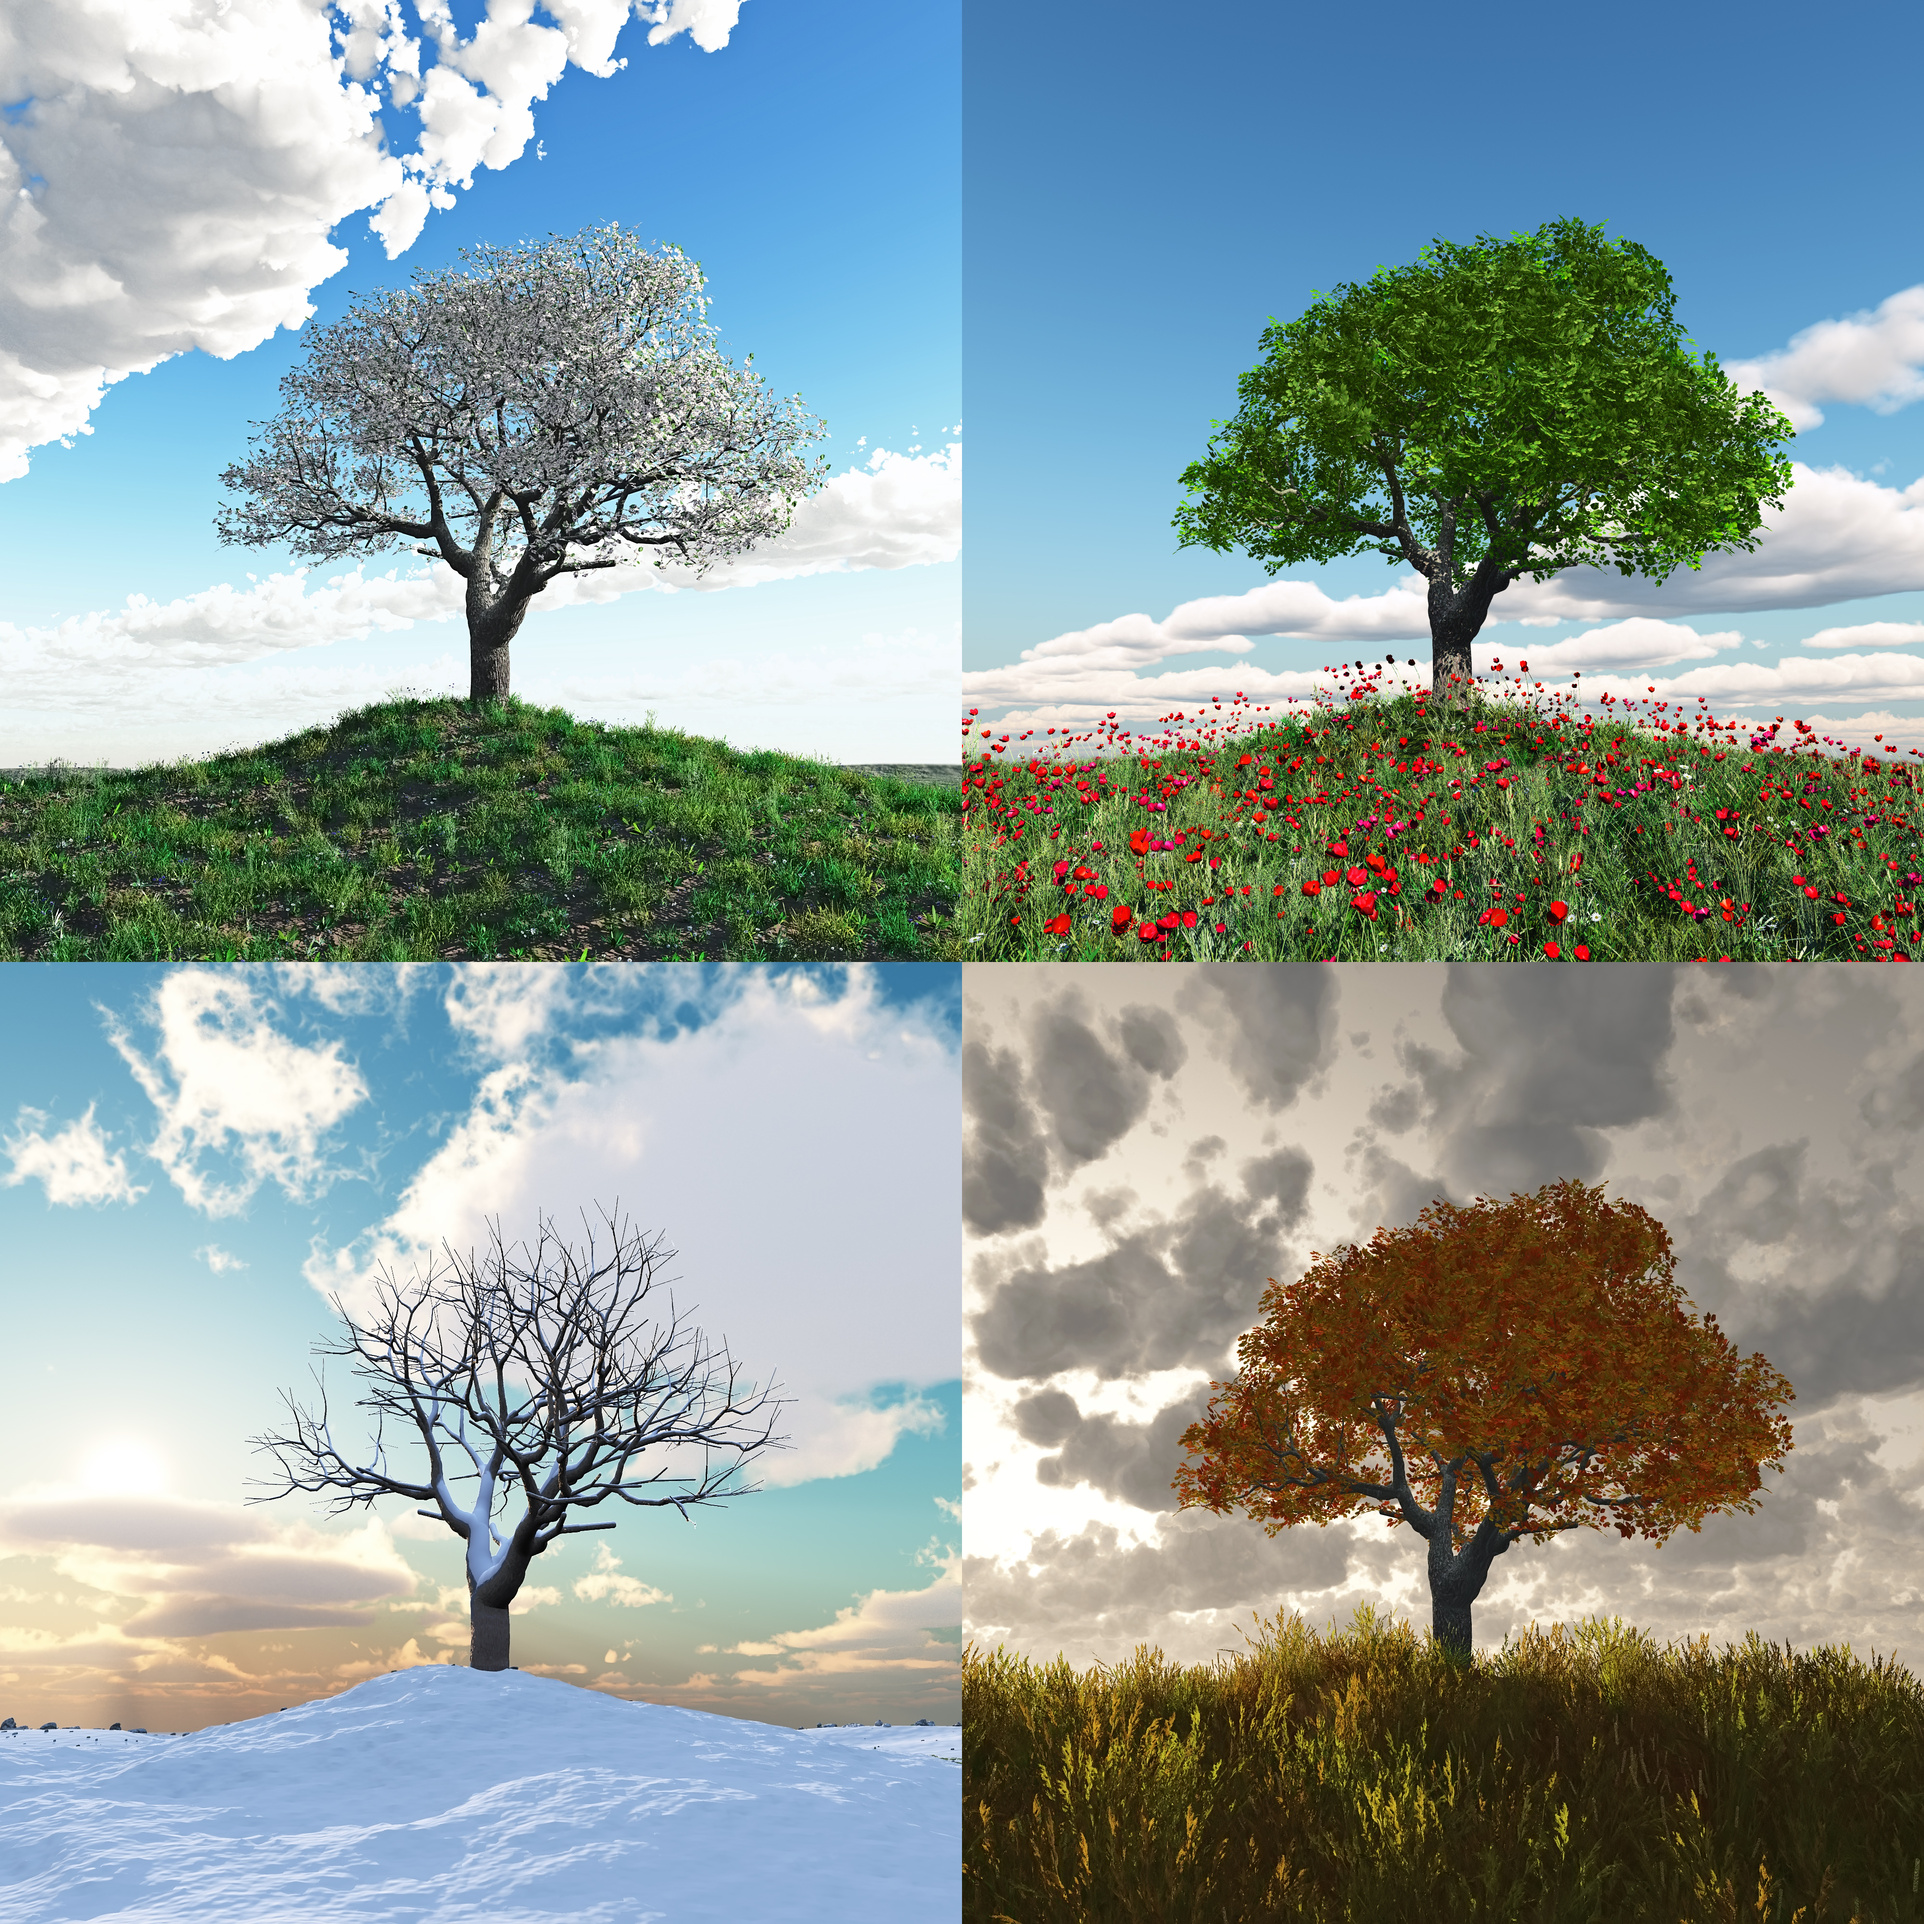
\includegraphics[width=0.5\linewidth]{quatre-saisons.jpg}
    \caption{les 4 saisons.}
    \label{fig:enter-label-1}
\end{figure}

\end{frame}


\begin{frame}{Principe}
\framesubtitle{Comment la prévision est faite?}

\begin{itemize}
    \item Calculer l'anomalie du modèle.
    \item déterminer les quantiles (1/3 , 2/3).
    \item projeter les ensembles.
\end{itemize}
\end{frame}

\begin{frame}{Principe}
\framesubtitle{Comment la prévision est faite?}
\begin{figure}
    \centering
    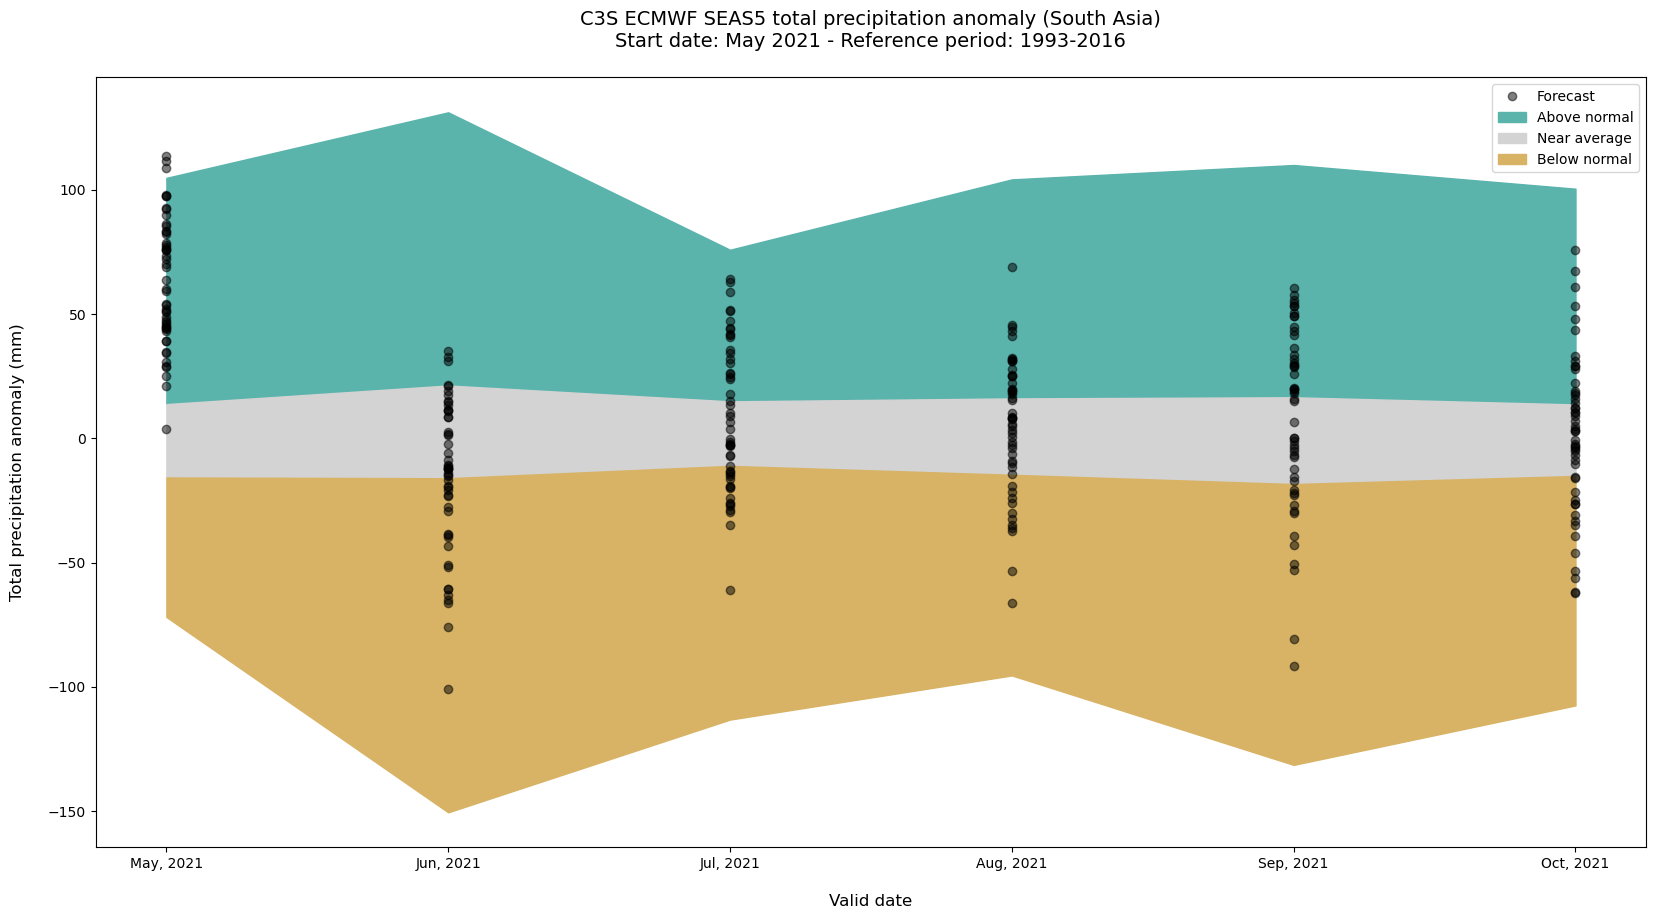
\includegraphics[width=0.8\linewidth]{sf_ensemble.png}
    \caption{Precipitation Forecast}
    \label{fig:enter-label}
\end{figure}
    
\end{frame}